\section{Experiences}
With the datasets and the classifiers in our hands, we can now start the actual trial phase. This will be done in three steps: first, we will go through some preliminary tests and observe how classifiers perform in each situation. These tests were created in order to fine tune the algorithms to improve their prediction power, such as scaling the input data, finding optimal parameters relative to the classifier or extracting the best features among the 119 of which our datasets are constructed. After that, thanks to the modularity of our ground truth generator, a variety of different dataset combinations will be produced and fed to the classifiers. Based on the results from the two previous steps, the goal of the third stage is to only keep the top K algorithms that offer satisfying outcomes, both in terms of accuracy and time, and proceed to final assertion tests. Although we were able to generate different kinds of datasets, we were however limited in the number of samples they contained depending on when the experiences were performed. Indeed, as explained in chapter \ref{methods}, we receive new samples on a daily basis and the analysis can take time. That is why the first experiments were run on smaller datasets to eventually reach around 140 000 samples for the economical analysis. Statistics regarding this adapted ground truth can be found in \autoref{gt_stats}. Eventually, the ground truth contained 43 different packers with more than 10 occurrences.


Before getting to the heart of the matter, we would like to explain how data is read and prepared for learning since this process is nearly always the same for the creation of any classifier. Let's look at the following code:

\begin{lstlisting}[language=python]
import pandas as pd

gt = pd.read_csv('../../dumps/various_sizes/1K.csv')
cols = [col for col in gt.columns if col not in ['label']]
data = gt[cols]
target = gt['label']
data_train, data_test, target_train, target_test = train_test_split(
        data, target,
        test_size = 0.20,
        random_state = 0 )
\end{lstlisting}

Since our datasets are saved in CSV files, we use the \texttt{pandas} library to read and store them in DataFrame structures by specifying the path to our dump folder on line 3. Line 4 retrieves all column names referring to the features. Line 5 stores all these values in a structure called \texttt{data} while the labels go in the \texttt{target} array. The next step is then to split our data between the training and test set using two arguments:
\begin{itemize}
    \item \textit{test\_size}: the purpose of splitting between a training and a test set is to verify the accuracy of our algorithms over fresh data while knowing the desired labels. Moreover, proceeding as such enables to ensure that we do not overfit because the predicted set is different that the one used for training. \textit{test\_size} represents the proportion of data that should be used for testing. Intuitively, 1 - \textit{test\_size} defines the amount of data kept for the training phase. Since in Data Science, at least three quarters of the time is spent on collecting and pre-processing the data, we decided to apply the Pareto principle and split between the training and the test set with a ratio of 80/20. We will always use this coefficient by default.
    \item \textit{random\_state}: the seed used to randomly distribute the data between the training and test set. Because the purpose of these experiments is to compare the results between algorithms on the same datasets and splits, deterministic values should be favored. That's why we keep the same seed of 0 among the different runs.
\end{itemize}

This being defined, we can now dive into the set of tests and analyze the generated outputs. For clarification, one should know that before proceeding to data variations, the datasets that will be used hereafter were generated using all detectors with an intermediate threshold of 3 over 5.

Please note that the following experiments were run either on our personal laptops or on a server with the following specifications: 2 cores running at 2.394 Hz, 4 GB of RAM.

\subsection{First phase: preliminary tests} \label{first_phase}
\paragraph{Control}
In order to get a rough first idea on how the classifiers behave, we simply tried them on a small dataset of only a thousand samples. Although no specific treatment was applied to the algorithms or the input data yet, this test is a good indicator to see which classifiers already stand out and how they will improve with further tuning. Figure \ref{fig:control} shows how well each classifier predict on the training and test set, a value of 1 corresponding to 100\% accuracy.
\begin{figure}[!ht]
  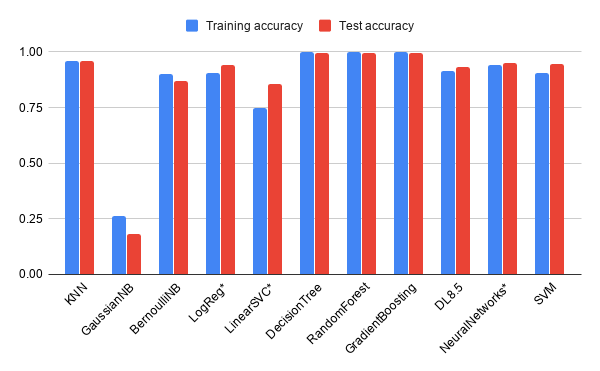
\includegraphics[width=\linewidth]{Figures/control.png}
  \captionsetup{justification=centering}
  \caption{Accuracies from running classifiers over 1000 samples without any tuning}
  \label{fig:control}
\end{figure}

While in average performances are located between 80 and 90\%, we can already identify poor and strong performers. The Decision Tree, the Ensembles of Decision Trees and the K-Nearest Neighbors algorithms already provide really promising outcomes without any tuning while Naive Bayes and Linear Models classifiers need customisation, especially the Gaussian distribution which does not even reach 20\% of precision on the test set.

Although tree-based algorithms seem to perform extremely well, these outcomes should be considered with some distance. Indeed, as they reach a 100\% precision over the training set, they might probably be overfitting. We will see in further sections how to solve this issue.

Some algorithms were marked with a star symbol next to their name on the X-axis. This means that they did not reach convergence, namely that the optimisation algorithm did not manage to come out with a coherent model based on the input data. The accuracies that are shown on the plot should then be treated with caution.

\paragraph{Data scaling} \label{data_scaling}

In section \ref{classifiers}, it has been explained that some algorithms might probably need the data to be pre-processed before starting the learning phase. The most common examples are the BernoulliNB and DL8.5 classifiers, which work with binary data while our datasets contain a mixture of both binary and continuous data. Without scaling, the outcomes are therefore meaningless. Therefore, one way to deal with bad performances or convergence issues might reside in data scaling. While algorithms working with trees pull their strength from the disparity of values to create their branches and leaves, other classifiers would need input data to fit within the same range in order to build a coherent prediction model.

K-Nearest Neighbors - hereafter KNN - works by computing distance between the different parameters and their values can be of any range. Some independent features may have a larger effect on the prediction capability of the algorithm and features with large values may not always be significant or may be biased. Therefore, it is wise to scale our data before fitting our model. One solution is to apply normalisation. By default, when we talk about normalisation, we actually refer to L2 normalisation. It is applied to each observation so that the values in a row have the same unit norm. This means that the sum of the elements is equal to 1. Figure \ref{fig:norma} illustrates the principle of normalisation using KNN with 10 neighbors.
\begin{figure}[ht]
\centering
    \begin{minipage}[b]{0.48\textwidth}
    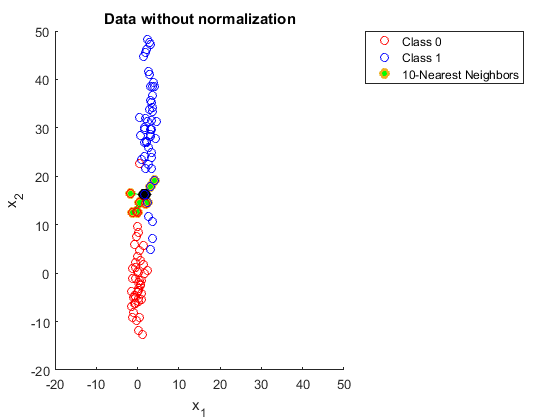
\includegraphics[width=\textwidth]{Figures/norma1.png}
\end{minipage}
\quad
\begin{minipage}[b]{0.48\textwidth}
    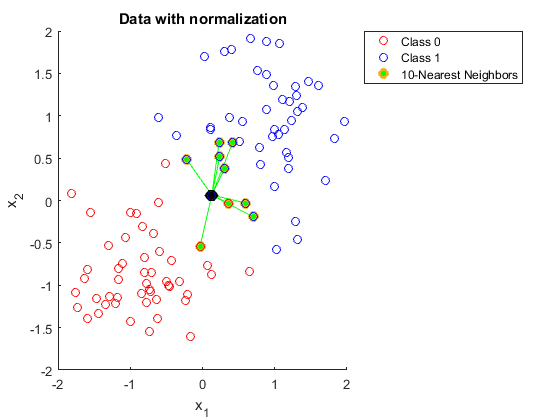
\includegraphics[width=\textwidth]{Figures/norma2.png}
\end{minipage}
\captionsetup{justification=centering}
\caption{Effects of normalisation using 10-Nearest Neighbors over a two class classification problem \cite{norma_source}}
\label{fig:norma}
\end{figure}

Naive Bayes classifiers also need the data to be preprocessed. Since the feature values could have any kind of variances and standard deviations, the assumed distribution could be spread out over a large range of values which will decrease the value of the probability density. Therefore, it makes sense to transform the attributes so that we end up with a mean of 0 and a standard deviation of 1. This process is called standardisation. Figure \ref{fig:norm_vs_stand} shows really succinctly how to understand the difference between normalisation and standardisation.
\begin{figure}[!ht]
\centering
  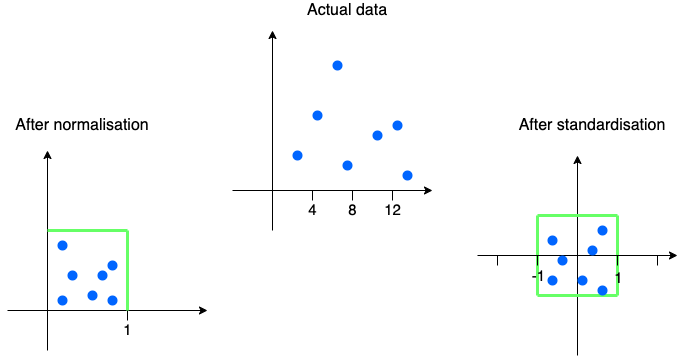
\includegraphics[width=\linewidth]{Figures/norm_vs_stand.png}
  \captionsetup{justification=centering}
  \caption{Basic representation of the concepts of normalisation and standardisation}
  \label{fig:norm_vs_stand}
\end{figure}
Regarding the Bernoulli classifier, we need an extra pre-processing step. Indeed, it assumes binary values while our dataset initially contains continuous data. Therefore, we first scale the data between [-1;1] using standardisation, and then use the value of 0 as the binary threshold. Feature values above 0 are replaced by 1 while the other ones get value 0.

Linear models do not necessarily need feature scaling. Worse, we might even loose the quantitative meaning of the coefficients. Therefore, our first approach was not to pre-process the data and observe how the classifier would behave. But as shown in the previous section, we suffered from convergence issues. This is the complete output we got from \texttt{scikit} when running the classifiers:
\begin{lstlisting}
/usr/local/lib/python3.7/site-packages/sklearn/linear_model/_logistic.py:940: ConvergenceWarning: lbfgs failed to converge (status=1):
STOP: TOTAL NO. of ITERATIONS REACHED LIMIT.

Increase the number of iterations (max_iter) or scale the data as shown in:
    https://scikit-learn.org/stable/modules/preprocessing.html
\end{lstlisting}

As the error message suggest, the \textit{max\_iter} parameter of the classifier should be increased because the optimisation algorithm did not manage to converge. This parameter controls the number of iterations taken for the solver to reach convergence, which is set to 100 by default. We therefore tried again with higher values, going from 1 000 to even a million of iterations, but we faced two issues. First, by increasing the number of iterations, as one could have guessed, the computation time also increased, going from a few milliseconds for the default case to a matter of seconds with a million of iterations. The second issue was that, even with these huge values, no convergence point could be found. We should not forget that we are only working with a dataset of 1 000 samples.
Our reflection was then that this diversity might be so strong that the classifier would need far more samples to reach convergence. But this cannot be measured at this point, so we eventually decided to scale our data the same way as we did for Naive-Bayes classifiers and see how it goes. This pre-processing was also applied to Kernelized Support Vector Machines since they are an extension of Linear Models.

Regarding Neural Networks, empirical researches showed that both scaling methods might be suited regarding the problem that need to be solved and the kind of dataset used. Comparing accuracies in both cases, we found out that applying standardisation was also the most suited option.

\begin{figure}[!ht]
  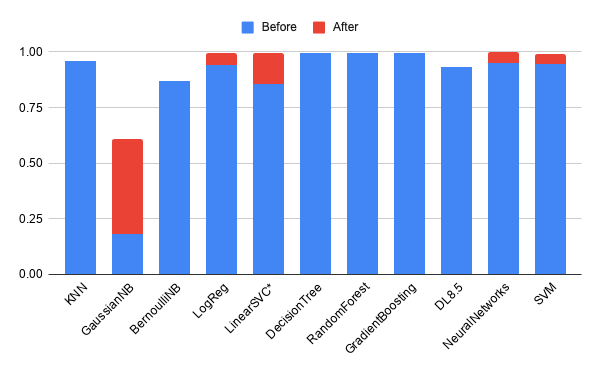
\includegraphics[width=\linewidth]{Figures/data_scaling.png}
  \captionsetup{justification=centering}
  \caption{Test accuracies from running classifiers over 1 000 samples with data scaling}
  \label{fig:data_scaling}
\end{figure}
Figure \ref{fig:data_scaling} acknowledges the importance of data scaling. While it doesn't change the test accuracy for some classifiers over 1 000 samples, others benefit a boost of prediction power, like Linear Models, Neural Networks or even the GaussianNB which upgrades from 18 to 61\% of precision. However, we still did not manage to get rid of convergence issue for the Linear Support Vector Machines - hereafter LinearSVC. 
Although these numbers are already promising, working with more samples and proceeding to parameters tuning might even further increase performances and allow to solve other issues like overfitting or non-convergence. This will be done in the next section.

\paragraph{Parameters tuning}

Using a dataset of 8 000 samples, we consider the most relevant parameters relative to each classifier to end up with the combination offering the best prediction power. Each classifier being correctly configured, we will then be able to proceed to feature extractions, component analysis and dataset variations. Let's have a closer look at each algorithm and perform some parameters tuning.

\begin{itemize}
    \item \textbf{K-Nearest Neighbors:} Two metrics were evaluated for this test:
    \begin{itemize}
         \item \textbf{Number of neighbors (k):} In order to have a first idea of how the classifier would behave with increasing numbers of neighbors, we restricted the range of values from 1 to 14. The reason behind this is also an anticipation of potentially high computation time with bigger further datasets. For each iteration, a new classifier has been created with the appropriate parameter and the accuracies were plotted in figure \ref{fig:neigh}.
        \begin{figure}[!ht]
        \centering
          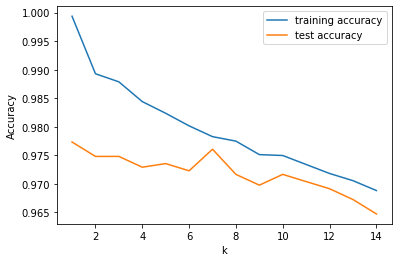
\includegraphics[width=0.80\linewidth]{Figures/neigh.png}
          \caption{Training and test accuracies for 1 to 14 Nearest Neighbors}
          \label{fig:neigh}
        \end{figure}
        Limiting the range to 14 was a good choice since both accuracies are globally decreasing with the increasing number of neighbors. We can also observe than the best trade-off between the training and test set performances corresponds to \textit{k=7}, which offers a better test accuracy than the default case of \textit{k=5}. One could argue why we do not just select a single neighbor since it gives a better training outcome. The reason is that this sweet spot might suffer from what we already referred to as  \textit{overfitting}. As introduced earlier, this happens when a model learns the detail and noise in the training data to the extent that it negatively impacts the performance of the model on the test data. This means that the noise or random fluctuations in the training data is picked up and learned as concepts by the model. In other words, the model is too specific and does not generalize well over new data. In order to reduce the likelihood of such event to occur, we rather choose a value of \textit{k} equal to 7.
        \item \textbf{Minkowski metric (p):} it defines the power parameter for the Minkowski metric which corresponds to the equation defining the distance between two points. A value of 2 is equal to using Euclidean distance while \textit{p=1} is the same as using the Manhattan distance. For higher values, the corresponding Minkowski distance is used. By varying this parameter, we mainly want to identify whether the Euclidean distance is fundamentally the best option. When looking at figure \ref{fig:minkowski}, using the Manhattan distance offers better results in both the training and the test situation. This distance equation should therefore be used in further experiments.
        \begin{figure}[!ht]
        \centering
          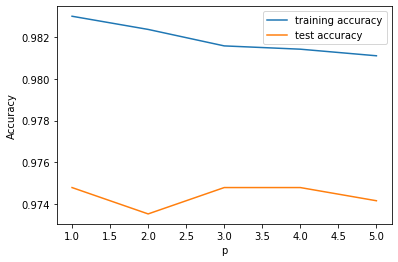
\includegraphics[width=0.80\linewidth]{Figures/minkowski.png}
          \captionsetup{justification=centering}
          \caption{Training and test accuracies for variation of the power parameter of the Minkowski metric}
          \label{fig:minkowski}
        \end{figure}
        
        From now on, the combination of parameters that will be used when initialising a new instance of our KNN classifier will be
\begin{lstlisting}[language=python]
KNeighborsClassifier(n_neighbors=7,p=1)
\end{lstlisting}
    \end{itemize}
    \item \textbf{Naive Bayes classifiers:} because of their probabilistic behaviour, Naive Bayes classifiers do not offer a lot of customisation. The only relevant parameter to adjust would be the \texttt{binarize} variable of the Bernoulli classifier, which has already been set up above.
    \item \textbf{Linear Models:}
    \begin{itemize}
        \item \textbf{Regularisation parameter (C):} Among the few parameters that Logistic Regression - hereafter LogReg - and LinearSVC classification offer, one retained our attention, namely the \textit{C} value, which corresponds to the inverse of the regularisation strength. The main goal of introducing regularisation in linear models is to avoid overfitting. The idea behind this concept is to try to minimise as much as possible the magnitude of the coefficients of \textit{w}, \textit{w} being the set of weights assigned to each feature (as explained in section \ref{LM}). It means that each feature should have as little effect as possible on the outcome, while still predicting well. Since the \textit{C} parameter represents the \textbf{inverse} of the regularisation strength, a higher value means less regularisation and vice-versa. In other words, with low values of \textit{C}, the model puts more effort to find \textit{w} coefficients close to 0 while when using higher values, the linear model will try to fit as best as possible to the training set, possibly resulting in overfitting.
    To find the \textit{C} value that suits the most our model, we tried different levels of magnitudes, going from 0.01 to 100, multiplying by 10 between each step. The resulting output for both classifiers is shown in figure \ref{fig:C_param}. The default value of 1 provides the best trade-off between both training and test set accuracy for LogReg while LinearSVC performs better with \textit{C=0.1}.
    \begin{figure}[ht]
    \centering
        \begin{minipage}[b]{0.45\textwidth}
        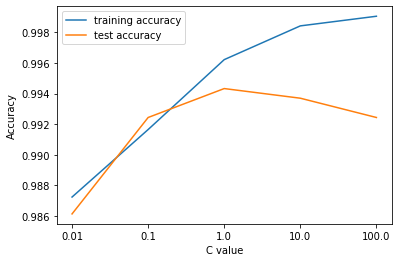
\includegraphics[width=\textwidth]{Figures/logreg.png}
    \end{minipage}
    \quad
    \begin{minipage}[b]{0.45\textwidth}
        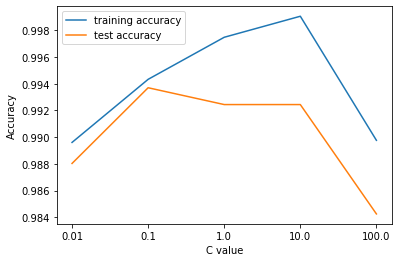
\includegraphics[width=\textwidth]{Figures/svc.png}
    \end{minipage}
    \captionsetup{justification=centering}
    \caption{Accuracies of LogReg (left) and LinearSVC (right) with different C values}
    \label{fig:C_param}
    \end{figure}
    \item \textbf{Loss function:} Specific to LinearSVC, this parameter specifies which loss function should be used in order to minimise the errors when finding the best boundary that will separate the data points in two classes. \texttt{scikit} offers two methods, namely \textit{hinge loss} and \textit{squared hinge loss}. Both are meant to be used for "maximum-margin" classification by support vector machines. The second function provides slightly better precision on the test set as shown on table \ref{Tab:linearsvc_loss}. Since this is the default method used by the classifier, we don't need to specify anything at initialisation.
    \begin{table}[h]
        \centering
         \begin{tabular}{|c|c|c|}
         \hline
         Type & Training acc & Test acc \\
         \hline\hline
         Hinge loss & 0.997  & 0.990\\
         \hline
         K-best & 0.997 & 0.992\\ 
         \hline
        \end{tabular}
        \caption{LinearSVC with different loss functions}
        \label{Tab:linearsvc_loss}
        \end{table}
    \end{itemize}
    These two linear model classifiers will thus be initialised as follows when running further tests:
\begin{lstlisting}[language=python]
logreg = LogisticRegression(random_state=0)
svc = LinearSVC(C=0.1, max_iter=10000, random_state=0)
\end{lstlisting}
    Note that we still need to increase the number of iterations to at least 10 000 for LinearSVC before reaching convergence. This implies that the training is already 3 times slower than the default case where \textit{max\_iter=100} while the dataset contains only 8 000 samples.
    \item \textbf{Decision Tree:} In \texttt{scikit}, decision trees come with a lot of relevant parameters that can be tuned. We retained the following:
    \begin{itemize}
        \item \textbf{Criterion:} The function used by the algorithm to measure the quality of a split in the tree, either the Gini impurity or the Information Gain. It appears that the default Gini criteria indeed worked better over our dataset.
        \item \textbf{Splitter:} Also relative to splitting, it represents the strategy that should be used to split between new branches at each node. The algorithm can either choose the "best" split, subdividing based on the current most relevant feature, or using the "random" strategy, which will simply randomly select one feature among all the possible ones and split it. This policy is more risky since the resulting tree might get deeper or loose precision. Anyway, the default "best" strategy showed more satisfying results.
        \item \textbf{Depth:} This parameter defines how profound the tree should be, namely how many levels it should have. If not defined, the nodes are expanded until all leaves are pure, meaning that no more splits are possible. While doing this not only ensures nearly perfect prediction over the input data, it also drastically increases the probability of overfitting and therefore bad generalisation over new data. Limiting the depth can therefore be judicious since deeper trees also imply higher computation times, which might not scale well with the further increasing number of samples. Figure \ref{fig:tree_depth} shows resulting accuracies for different depth levels.
        \begin{figure}[!ht]
        \centering
          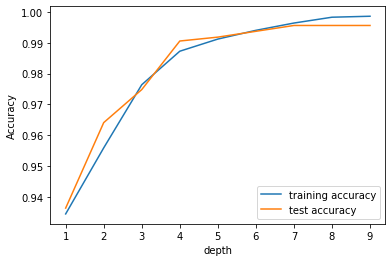
\includegraphics[width=0.80\linewidth]{Figures/tree_depth.png}
          \captionsetup{justification=centering}
          \caption{Training and test accuracies of the Decision Tree classifier for different depths}
          \label{fig:tree_depth}
        \end{figure}
        As we can see from the plot, increasing the depth improves both accuracies up to a certain point where the test results are constant. The best result obtained starts at depth 7, which offers a good compromise between the two accuracies and reduces the risk of overfitting.
        \item \textbf{Number of samples:} the samples in a tree can be used in two approaches: either to set up the minimum number of samples required to split an internal node, either the minimum amount of samples that should appear in each leaf node. Performances were at their climax with \textit{min\_samples\_split = 10} and \textit{min\_samples\_leaf = 7}.
    \end{itemize}
    All in all, the decision tree classifier will be initialised as follows:
\begin{lstlisting}[language=python]
decision_tree = DecisionTreeClassifier(max_depth=7,
                min_samples_split=10,
                min_samples_leaf=7,
                random_state=0)
\end{lstlisting}   
    \item \textbf{DL8.5:} As it is also a tree algorithm, this classifier has common parameters with decision trees but also has its own:
    \begin{itemize}
        \item \textbf{max\_depth:} It allows to define the maximum depth of the tree to be learned. Although this depth improves the results, it seriously deteriorates the performance - see figure \ref{fig:dl8.5}. Indeed, when the depth increases, the accuracy improves but we suffer a huge time overhead. Moreover, we quickly find ourselves saturating the RAM of our computer which causes a complete system crash.
        \begin{figure}[!ht]
        \centering
          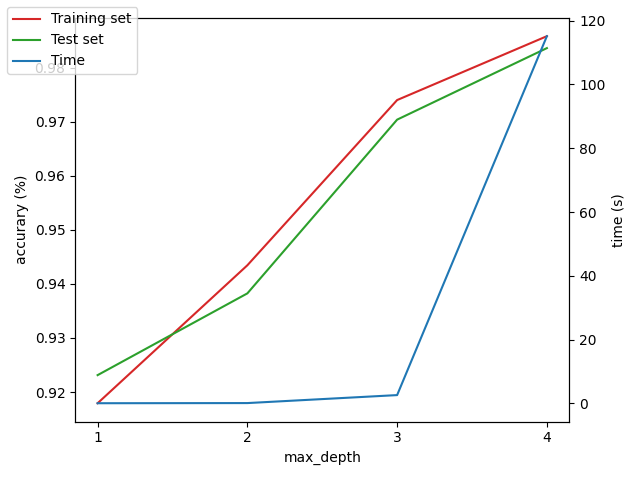
\includegraphics[width=0.80\linewidth]{Figures/dl8.5.png}
          \captionsetup{justification=centering}
          \caption{Training and test set accuracies for different depths with their respective learning times}
          \label{fig:dl8.5}
        \end{figure}
        \item \textbf{min\_sup:} Specifies the minimum number of examples in the training data that every leaf should cover. In our case, the variation of this value did not change the accuracy.
        \item \textbf{iterative:} A boolean value to use a \textit{Breadth-first search} instead of a \textit{Depth-first search}. Once again, no variation in precision between the two possibilities.
        \item \textbf{time\_limit:}: As its name suggests, it allows to set a time limit for the execution of the classifier.
    \end{itemize}
    This algorithm consumes a lot of RAM and our computers did not have enough memory, so we limited the depth to 3 and the computation time to 120 seconds. These values allow the algorithm to stop just before saturating our memory.
    \item \textbf{Ensembles of Decision Trees:} As their name indicates, Ensembles of Decision Trees are made of multiple Decision Trees and thus inherit their parameters. However, they also have another characteristic relative to the ensemble itself that can be tuned, namely the number of estimators. Pretty straightforward, it specifies the number of trees in the ensemble. The more trees are added, the more efficient the classifier become, but this is done at the expense of the computation time. By looking at the first graph from figure \ref{fig:ensemble_n_trees}, we see that we obtain the same test accuracy with 170 or more trees but also with 35 estimators for the Random Rorest. The difference is that it took 23 ms to reach the latter with a depth of 5 while 1.1s was required to reach 170 components. Regarding the Gradient Boosted classifier on the right-hand side plot, we can also notice that starting from 35 estimators, the prediction power stays constant. With such amount of trees and a limited depth of 5, it took 2.92s to train the algorithm while the default value of 100 trees needed more than 8s.
    \begin{figure}[ht]
    \centering
        \begin{minipage}[b]{0.45\textwidth}
        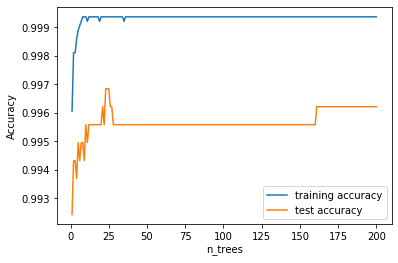
\includegraphics[width=\textwidth]{Figures/randomforest_trees.png}
    \end{minipage}
    \quad
    \begin{minipage}[b]{0.45\textwidth}
        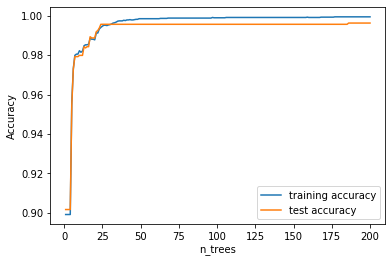
\includegraphics[width=\textwidth]{Figures/gradientboosted_trees.png}
    \end{minipage}
    \captionsetup{justification=centering}
    \caption{Accuracies of Random Forest (left) and Gradient Boosting (right) classifiers with varying number of trees}
    \label{fig:ensemble_n_trees}
    \end{figure}
    
%     Here below are shown the final combination of parameters for both ensembles of decision trees:
% \begin{lstlisting}[language=python]
% forest = RandomForestClassifier(n_estimators=35,
%                             max_depth=5,
%                             random_state=0)
% gradient = GradientBoostingClassifier(n_estimators=35,
%                             max_depth=5,
%                             random_state=0)
% \end{lstlisting}
    %cf annexe pour plus en profondeur
    \item \textbf{Neural Networks:} The MLP classifier that we use as part of the Neural Networks family embeds many different parameters. We can for example mention the activation function used between the hidden layer or the solver used for optimisation. The thing is that for these parameters, no matter the range of values tested, the default case always showed the best results.
    
    One parameter still attracted our attention, namely the \textit{hidden\_layer\_sizes}. Represented by a tuple, it allows to specify the number of desired hidden layers for the MLP classifier and how many neurons should lay in each layer. There is no rule of thumb to know neither the number of layer nor the number of neurons. Therefore, we tried all possible combinations of layers from length 1 to 4 made out of \textit{25, 50, 75} and \textit{100} neurons such that computation times would stay in a reasonable bound. Figure \ref{fig:mlp_HL} shows all possibilities. Note that the legend for the X-axis was removed for readability due to the high number of combinations. From left to right, the number of hidden layers as well as their density decrease along this axis.
    \begin{figure}
    \centering
      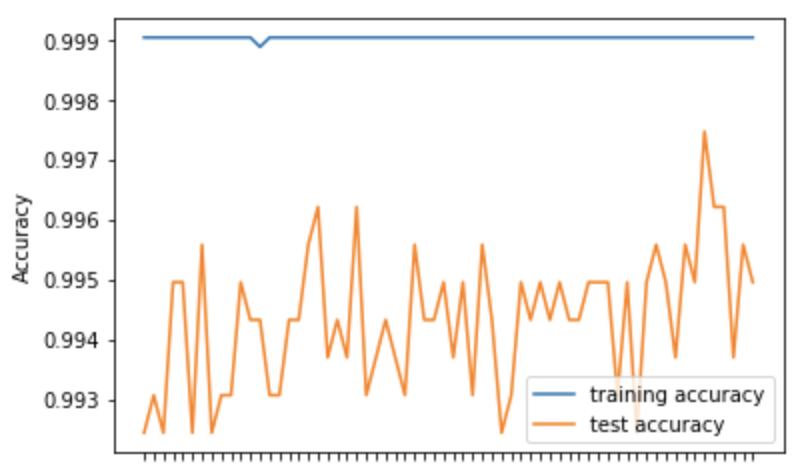
\includegraphics[width=0.80\linewidth]{Figures/mlp_HL.png}
      \captionsetup{justification=centering}
      \caption{Training and test accuracies of the MLP classifier for different hidden layers combinations}
      \label{fig:mlp_HL}
    \end{figure}
    As we can see, the results do not follow any kind of linear curve which means that increasing the layers or neurons do not necessarily imply better outcomes. However, one point stands out of the crowd and reaches a test accuracy of 99.7\%, which corresponds to the \textit{(75,100)} combination.
    \item \textbf{Support Vector Machine:} In addition to the regularisation parameter also offered by Linear Models, parameter customisation of the SVM relies on which kernel is used by the classifier. Understanding exactly how each kernel works is out of the scope of this work, but one should simply retain that they differ in the way they mathematically map the data from one space to a new multidimensional domain, the \textit{linear} kernel using a linear hyperplane while \textit{rbf} and \textit{poly} use non-linear ones. As we can see from figure \ref{fig:svm_kernel}, the default \textit{rbf} kernel performs the best.
    \begin{figure}
    \centering
      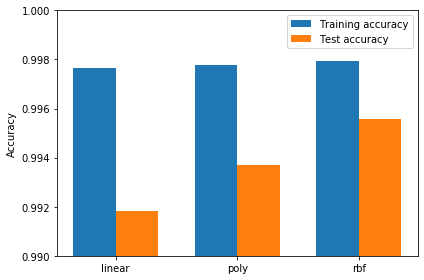
\includegraphics[width=0.80\linewidth]{Figures/svm_kernel.png}
      \captionsetup{justification=centering}
      \caption{Training and test accuracies of the SVM classifier for different kernels}
      \label{fig:svm_kernel}
    \end{figure}
    Therefore now, parameters relative to the kernel can be tuned, like the kernel coefficient or if the shrinking heuristic, which can sometimes shorten the training time, should be used. Once again, all default parameter values were the most fitted. We ended up having the same classifier as without parameter tuning but we however have the confirmation that the right kernel was used.
\end{itemize}

\begin{figure}[]
\centering
  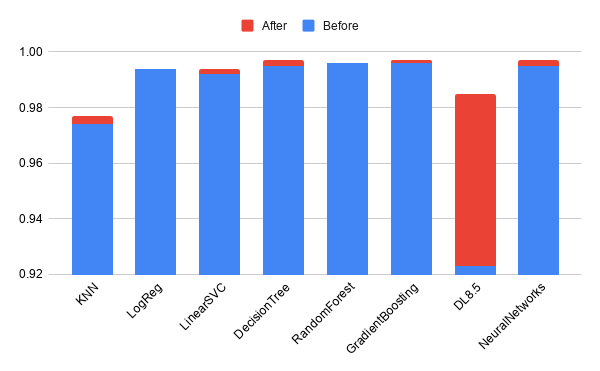
\includegraphics[width=0.80\linewidth]{Figures/parameter_tuning.png}
  \caption{Test accuracies before and after parameters tuning}
  \label{fig:param_tuning}
\end{figure}
Figure \ref{fig:param_tuning} is a summary that shows how parameters tuning impacted test accuracies over the dataset of 8 000 samples used in this section (the Naive Bayes classifiers and SVM were removed since no customisation was performed or because they kept their default parameters).

While some classifiers slightly increase their prediction power, others kept the same accuracy. Still, they did improve. Indeed, both Linear Models got rid of their convergence issue while other already efficient algorithms, such as Decision Tree and Ensembles of Decision Trees, improved in terms of computation time because of depth limitation.
DL8.5 improved by more than 6\% but under time constraints, since such outcome was obtained by letting the algorithm run for two entire minutes.
Nevertheless, we can conclude that parameters tuning enhanced, although moderately, overall performances.

\paragraph{Feature relevance}

Working with less than the total number of available features might slightly weaken performances while significantly decreasing the training time. In order to verify this assumption, we used two different techniques to select the best features among the initial 119, over a dataset of 16 000 samples:
\begin{itemize}
    \item \textbf{K-best:} Extracting the K best features out of the initial model
    \item \textbf{Iterative process:} Extracting the K best features from the model for different increasing sizes of the test set. The intersection of the best features is kept over the iterations.
\end{itemize}

For both methods, we use the \texttt{SelectFromModel} function from \texttt{scikit} to retrieve the best features out of the model. This methods has a parameter called \textit{threshold} which is relative to the importance of the feature in the model. We therefore tried different values in order to widen the possible combination of features. To select the best features set for each scenario, we proceeded as follows: for each threshold, only keep the set of features if the accuracy on the test set is no more than 5\% worse than the default case where all the features are kept. All candidates satisfying this requirement are added to a list with their time and corresponding accuracy. At the end, we iterate over this list and compute an indicative \textit{time-to-accuracy ratio}, which is just the division of the percentage of time saved by the percentage of test accuracy lost. The best features set for \textbf{K-best} and \textbf{Iterative process} is eventually output. Note that \texttt{SelectFromModel} only works with estimators that have a \texttt{coef\_} or \texttt{feature\_importances\_} attribute after fitting. Therefore, only some classifiers are eligible to this feature selection experiment, namely Linear Models, Decision Tree and Ensemble of Decision Trees.

In order to get a rough idea of the weight of each feature in the decision process, an interesting preliminary step is to take a look at their spread in terms of coefficients magnitude for Linear Models and feature importance for Trees. All the plots can be found in figures \ref{fig:fs_logreg} to \ref{fig:fs_randomforest}.

Regarding LogReg and LinearSVC, the coefficient associated with each feature in the linear function can be retrieved. The higher the coefficient, the higher the importance of a feature. By looking at the plots in figures \ref{fig:fs_logreg} and \ref{fig:fs_linearsvc}, what first stands out is that there is a lot of disparity in the magnitude of the coefficients. Some are close to 0 thanks to regularisation, and on average, nearly all the coefficients have a value between -1 and 1 for the first model while in the range of -0.3 and 0.3 for the latter. However, the shape of the spread is the same. We then infer that in these models, almost every coefficient has its importance in the decision process and we cannot discern a small subset of features that could explain the entire model on their own. Therefore, a first hypothesis would be to assume that feature selection process should not reject a lot of features.

When it comes to trees, the matter is not to evaluate the magnitude of the coefficients in any linear equation, but rather evaluating the power of each feature to perform splitting. It is calculated as the decrease in node impurity weighted by the probability of reaching that node. The node probability can be calculated by the number of samples that reach the node, divided by the total number of samples. The higher the value, the more important the feature. When looking at the plots in figures \ref{fig:fs_tree} and \ref{fig:fs_gradientboosted}, we can observe that out of the 119 features, only 25\% are actually used by the classifiers and the 4 same attributes are able to define more than 75\% of the models, namely features 26, 39, 47 and 84. It might therefore be legitimate to anticipate that by applying feature selection, the domain of attributes will be significantly reduced, resulting in possibly huge time savings. For the Random Forest, the dispersion is less impressive, as show in \autoref{fig:fs_randomforest}. Although a few features are completely neglected by the classifier, most of them have an importance that lies between 0 and 0.05. We can also identify outsiders, but they "only" define 20\% of the model. Proceeding to feature selection over this classifier will still be relevant, but will probably result in less drastic changes than other tree classifiers. Nevertheless, we can remark that for these three classifiers, one feature always significantly defines the majority of the model, namely feature 47. This feature, as described in
\autoref{extracted_features}, represents the entropy of the entire PE file. This observation confirms the importance of entropy in the context of packed malware detection, as demonstrated by Lyda et al. \cite{lyda_using_2007}.

A summary of the feature relevance process is shown in table \ref{Tab:fs_table} while specific results for each classifier can be found in tables \ref{Tab:tab_logreg} to \ref{Tab:tab_randomforest}.

\begin{table}[H]
    \centering
    \resizebox{\textwidth}{!}{%
     \begin{tabular}{|c|c|c|c|c|}
     \hline
     Classifier & Selection & \# features & Ratio & Final test acc.\\
     \hline\hline
     LogReg & K best & 84 & 241.80 & 0.9897\\
     \hline
     LinearSVC & K best & 51 & 362.50 & 0.9878\\ 
     \hline
     Decision Tree & K best & 17 & 293.27 & 0.9866\\ 
     \hline
     Gradient Boosted & K best & 21 & 260.50 & 0.9922\\ 
     \hline
     Random Forest & Iterative & 23 & 256.37 & 0.9885\\ 
     \hline
    \end{tabular}%
    }
    \caption{Best results for feature selection based on ratio value}
    \label{Tab:fs_table}
\end{table}
A first observation that can be made is that indeed, feature selection appeared to be beneficial for every tested classifier since all ratios are positive. The ratio is a good indicator of how much feature selection impacted the performance. Because it divides the time by the accuracy, a higher ratio value means that either the fitting was faster, either that the loss of precision was limited. As an example, Decision Tree has a ratio of 293.27, which means that, compared to the default case with all features kept, it lost 0.158\% of prediction power while reducing the computation time by 46.257\%. On the other hand, Logistic Regression "only" improved its computation time by 22.83\% while losing 0.094\% of precision the test set, which results in a lower ratio of 241.8012.

Despite such good numbers, one should remark that both the LinearSVC and the Gradient Boosted classifiers are quite slow in terms of training time. While all the other algorithms are in the order of a few tens of milliseconds, these two still need between 1 and 3 seconds to reach convergence after feature selection. Regarding LinearSVC, it is explained by the high number of iterations required to reach convergence, which obviously slows down the process.

Another deduction that can be drawn relates in the kind of feature selection process used. Four classifiers out of five functioned better employing the K best feature extraction. Finding the best intersection between several sets made out of different test size did not outperform its static version. Moreover, the fixed cost of finding the best subset of feature is always higher for the iterative process.

Last but not least, the assumptions about the resulting amount of features have been confirmed. While the Linear Models kept a majority of attributes, the tree-based models managed to issue impressive outcomes by retaining only around 14 to 19\% of the domain.

As a conclusion for this experiment, we can assert that applying feature selection to linear and tree-based models is indeed relevant since the prediction power still lies around 99\% while the computation time was drastically decreased, as shown by the ratio coefficient. Such time savings are precious and could be used to improve other variables, like dataset customisation or sharper tuning of other parameters specific to the classifiers. We could think of the depth limitations for the trees that was limited due to time constraints which could know probably be raised.

\paragraph{Principal Components Analysis}

Also referred to as PCA, this technique fulfills the same objective as the previous test, which is reducing the dimension of the feature space. The difference is that this method doesn't remove any features but instead groups them to create new components, as shown in figure \ref{fig:PCA}. Each component is an independent new linear combination of some features. They are ranked by importance weights which means that a variation of the first component has more impact on the overall model than the same variation over the second component. In short, the goal of PCA is to identify directions (or principal components) along which the variation in the data is maximal. 
\begin{figure}[!ht]
\centering
  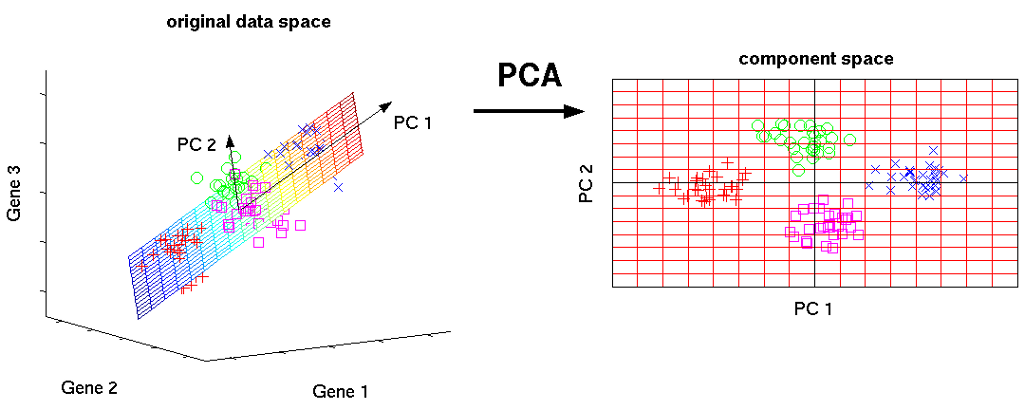
\includegraphics[width=0.80\linewidth]{Figures/PCA.png}
  \caption{Reduction of the dimensional feature space from 3 to 2 \cite{pca_source}}
  \label{fig:PCA}
\end{figure}
\texttt{scikit} already implements PCA with different customisation parameters, like the amount of variance that need to be explained by the resulting model or the number of components that should be kept. We went for the second option. In order to elect the best set of components, we computed the 119 combinations over a dataset of 16 000 samples and only retained the ones improving the computation time. Then, the 5 sets presenting the best accuracies were selected.

The following table summarises the best results we got from running PCA over the dataset before learning with the different algorithms. Complete plots and tables relative to each classifier can be found in figures \ref{fig:knn_pca} to \ref{fig:svm_pca}. Note that since PCA requires data standardisation as a part of its components analysis, DL8.5 is not eligible to this process due to its binary data requirement.


\begin{table}[H]
    \centering
    \resizebox{\textwidth}{!}{%
     \begin{tabular}{|c|c|c|c|c|c|}
     \hline
     Classifier & \# components & Test accuracy & Time (s)\\
     \hline\hline
     KNN & 71 & 0.994389 \cellcolor{green}(+1.50\%) & 0.0780669 (-33.07\%)\\
     \hline
     GaussianNB & 28 & 0.949813 \cellcolor{green}(+60.62\%) & 0.0159705 (-28.83\%)\\ 
     \hline
     BernoulliNB & 19 & 0.948254 \cellcolor{green}(+7.83\%) & 0.235989 (-22.17\%)\\
     \hline
     LogReg & \cellcolor{yellow}109 & 0.99096 (+0.031\%) & 0.376064 (-3.75\%)\\
     \hline
     LinearSVC* & \cellcolor{yellow}109 & 0.990025 (+0.032\%) & \cellcolor{orange}5.93549 (-18.56\%)\\
     \hline
    DecisionTree & 15 & 0.982855 \cellcolor{red}(-0.54\%) & 0.180111 (-26.58\%)\\
    \hline
    GradientBoosted & 33 & 0.990648 \cellcolor{red}(-0.44\%) & \cellcolor{orange}5.78071 (-2.58\%)\\
    \hline
    RandomForest & 7 & 0.973815 \cellcolor{red}(-1.60\%) & 0.338177 (-21.13\%)\\
    \hline
    MLP & \cellcolor{yellow}104 & 0.996259 (+0.22\%) & \cellcolor{orange}3.40213 (-33.30\%)\\
    \hline
    SVM & \cellcolor{yellow}104 & 0.995324 (+0\%) & \cellcolor{orange}1.39707 (-11.97\%)\\
    \hline
    \end{tabular}%
    }
    \captionsetup{justification=centering}
    \caption{Top 1 results from applying PCA, then keeping only iterations improving time and eventually sorting by accuracies}
    \label{Tab:pca_table}
\end{table}

Although computation times improved in every case, PCA does not seem to be suited for every classifier. Indeed, while KNN and Naive Bayes classifier benefit from a significant improvement in terms of accuracy, tree-based models endure a loss of prediction power. A probable reason for that is that trees derive their cogency from the diversity of features, allowing to split between branches more easily. Therefore, applying PCA reduces the dimensionality of the data and creates abstract data, namely linear combinations of the original features, resulting in harder interpretations by the models.

Regarding the other algorithms, they boosted their precision by a few hundredths but when looking at their corresponding number of components, we can see that PCA did not manage to gather a lot of features together. However, these outputs are comprehensible. Since the classifiers used in these situations - Linear Models, SVM and MLP - already try to find an optimal combination of weights that fits the feature values, applying PCA in addition does not really make sense as the core idea is pretty much the same. PCA could rather be seen as a refinement step than an actual improvement for these models.

Apart from the procedure of components analysis itself, we remark that, as after applying feature selection, both the LinearSVC and Gradient Boosted classifier have computation times in the order of several seconds. Despite less intense, the MLP and SVM classifiers fit in the same order of magnitude. Regarding LinearSVC, the time explosion can be justified as in the previous section, but the thing is that, as the star symbol in the table states, no convergence was reached this time.

In the end, a conclusion would be to say that apart from the KNN and Naive Bayes classifiers, applying PCA as a pre-processing step to the data did not show enough persuasive results to be implemented.

% \paragraph{Time analysis}

% This last primary test is a first step towards a more complete economical analysis that will be performed at the very end of our experiments. This is done at a smaller scale to have a preliminary intuition on how classifiers behave over time and if they maybe need to be retrained. Each algorithm is fed with datasets of different sizes mimicking the training duration (from one week to an entire month) and has to predict the labels of a new input set that has been generated two months after the initial learning. The main objective of this test is to verify if the model is stable over time.

% Table \ref{Tab:time_analysis} gathers the different test accuracies obtained for different training periods.

% \begin{table}[H]
%     \centering
%     \resizebox{\textwidth}{!}{%
%     \begin{tabular}{|c|c|c|c|c|c|}
%     \hline
%     Classifier & 1 weeks & 2 weeks & 3 weeks & 1 month\\
%     \hline\hline
%     KNN & 0.915 & 0.941 & 0.943 & 0.955\\
%     \hline
%     \rowcolor{red}
%     GaussianNB & 0.543 & 0.547 & 0.547 & 0.505\\
%     \hline
%     \rowcolor{red}
%     BernoulliNB & 0.562 & 0.513 & 0.452 & 0.45\\
%     \hline
%     LogReg & 0.986 & 0.986 & 0.982 & 0.982\\
%     \hline
%     LinearSVC* & 0.981 & 0.984 & 0.981 & 0.98\\
%     \hline
%     \rowcolor{green}
%     DecisionTree & 0.919 & 0.92 & 0.987 & 0.989\\
%     \hline
%     \rowcolor{green}
%     GradientBoosted & 0.978 & 0.986 & 0.988 & 0.988\\
%     \hline
%     \rowcolor{green}
%     RandomForest & 0.984 & 0.981 & 0.981 & 0.984\\
%     \hline
%     \rowcolor{red}
%     DL8.5 & 0.873 & 0.698 & 0.698 & 0.699\\
%     \hline
%     MLP & 0.979 & 0.981 & 0.985 & 0.984\\
%     \hline
%     SVM & 0.984 & 0.982 & 0.986 & 0.987\\
%     \hline
%     \end{tabular}%
%     }
%     \caption{Time analysis for different classifiers over datasets with the threshold set to 3/5}
%     \label{Tab:time_analysis}
% \end{table}

% Once again, the outcomes are contrasted. While it is pretty straightforward that Naive Bayes classifiers and DL8.5 do not generalize well over freshly new input data, other algorithms do not overfit and maintain stability over time. In general, the longer the training period, the better the prediction power. 

% Otherwise, we can draw two more conclusions. First, tree-based models confirmed their attractiveness since they provide the overall best performances and are more and more prone to be selected among the best classifiers. Secondly, LinearSVC did yet again suffer from convergence issue when learning over different periods of time and conversely reduced its probability to be kept for further work.

% These results are yet pretty convincing for the forthcoming economical analysis that will be performed over larger periods of time.

\subsection{Second phase: dataset variations}

The tests that were previously made mainly targeted the classifiers themselves and how the data had to be parsed in order to obtain the best performance. Now, since these parameters have been tuned, we can have a closer look at how datasets could be generated in a way that allows the models to extract as much information as possible. Thanks to our modular ground truth generator, we were able to produce different kinds of datasets with different characteristics, all containing 16 000 entries. The objective is to establish whether changing the way data are presented can have a positive impact on performance. Below we explain the kind of generated datasets and show how classifiers performed when using them as training data. 
\begin{itemize}
    \item \textbf{Threshold variation:} how many detectors out of 5 should at least agree before a sample is tagged with the label \textit{packed}. Table \ref{Tab:thresholds} shows the test accuracy per classifier using the different thresholds.
    \begin{table}
    \centering
    \resizebox{\textwidth}{!}{%
    \begin{tabular}{|c|c|c|c|c|c|}
    \hline
    Classifier & 1/5 & 2/5 & 3/5 & 4/5 & 5/5\\
    \hline\hline
    KNN & 0.956 & 0.972 & 0.981 & 0.987 & \cellcolor{green}0.988\\
    \hline
    GaussianNB & 0.768 & 0.675 & 0.907 & 0.953 & \cellcolor{green}0.974\\
    \hline
    BernoulliNB & 0.881 & 0.942 & 0.945 & 0.987 & \cellcolor{green}0.993\\
    \hline
    LogReg & 0.948 & 0.987 & 0.992 & \cellcolor{green}0.998 & 0.997\\
    \hline
    LinearSVC & 0.951* & 0.983* & 0.993 & \cellcolor{green}0.998 & 0.997\\
    \hline
    Decision Tree & 0.972 & 0.991 & 0.995 & \cellcolor{green}0.996 & \cellcolor{green}0.996\\
    \hline
    DL8.5 & 0.954 & 0.985 & 0.992 & \cellcolor{green}0.994 & 0.993\\
    \hline
    Gradient Boosted & 0.980 & 0.996 & 0.997 & \cellcolor{green}0.998 & \cellcolor{green}0.998\\
    \hline
    Random Forest & 0.966 & 0.993 & 0.994 & \cellcolor{green}0.998 & \cellcolor{green}0.998\\
    \hline
    MLP & 0.977 & 0.996 & 0.996 & \cellcolor{green}0.998 & \cellcolor{green}0.998\\
    \hline
    SVM & 0.978 & 0.995 & 0.996 & \cellcolor{green}0.997 & \cellcolor{green}0.997\\
    \hline
    \end{tabular}%
    }
    \caption{Threshold variation}
    \label{Tab:thresholds}
    \end{table}
    As we can see from the green cells, we achieve the best performance with a threshold of 5 detectors for 8 out of the 11 classifiers. This can probably be explained because smaller threshold values are too imprecise to come up with a decision while thresholds starting from 3 to 5 are more restrictive and therefore result in a more precise learning. It is also interesting to notice that the prediction power is often really similar for the two last threshold values, which means that if four detectors agree that a malware is packed, then the last one probably also does. Another point to raise is that in the case of the LinearSVC model, we see that using more flexible thresholds generates convergence issues. Using more strict thresholds is therefore a way to limit the probability of such event to occur.
    All in all, the threshold value that should be as restraining as possible.
    \item \textbf{Detector relevance:} 5 new datasets are generated without the outputs of one of the detectors. The goal of this test is to observe the weight of each detector in the decision process. The columns in table \ref{Tab:detectors} assigned with a detector name mean that this packer is removed from the decision process. Accuracies displayed are once again obtained over the test set with a threshold of 3/5.
    \begin{table}
    \centering
    \resizebox{\textwidth}{!}{%
    \begin{tabular}{|c|c|c|c|c|c|c|}
    \hline
    Classifier & All & DIE & Cisco & Manalyze & PEiD & PEframe\\
    \hline\hline
    KNN & \cellcolor{cyan}0.981 & \cellcolor{red}0.979 & \cellcolor{green}0.987 & \cellcolor{green}0.982 & \cellcolor{green}0.990 & \cellcolor{green}0.988\\
    \hline
    GaussianNB & \cellcolor{cyan}0.907 & \cellcolor{red}0.894 & \cellcolor{red}0.889 & \cellcolor{green}0.910 & \cellcolor{green}0.917 & \cellcolor{green}0.940\\
    \hline
    BernoulliNB & \cellcolor{cyan}0.945 & \cellcolor{red}0.942 & \cellcolor{green}0.985 & \cellcolor{red}0.940 & \cellcolor{red}0.987 & \cellcolor{green}0.992\\
    \hline
    LogReg & \cellcolor{cyan}0.992 & 0.992 & \cellcolor{green}0.994 &\cellcolor{green} 0.994 & \cellcolor{green}0.997 & \cellcolor{green}0.998\\
    \hline
    LinearSVC & \cellcolor{cyan}0.993 & 0.993 & \cellcolor{green}0.994 & \cellcolor{green}0.994 & \cellcolor{green}0.997 & \cellcolor{green}0.998\\
    \hline
    Decisio nTree & \cellcolor{cyan}0.995 & \cellcolor{red}0.993 & \cellcolor{green}0.996 & \cellcolor{green}0.996 & \cellcolor{red}0.994 & \cellcolor{red}0.988\\
    \hline
    DL8.5 & \cellcolor{cyan}0.992 & \cellcolor{red}0.988 & \cellcolor{green}0.994 & \cellcolor{red}0.991 & 0.992 & \cellcolor{green}0.994\\
    \hline
    Gradient Boosted & \cellcolor{cyan}0.997 & \cellcolor{red}0.996 & \cellcolor{red}0.996 & 0.997 & 0.998 & \cellcolor{green}0.999\\
    \hline
    Random Forest & \cellcolor{cyan}0.994 & \cellcolor{red}0.993 & \cellcolor{green}0.996 & 0.994 & \cellcolor{green}0.998 & \cellcolor{green}0.999\\
    \hline
    MLP & \cellcolor{cyan}0.996 & 0.996 & \cellcolor{green}0.997 & \cellcolor{red}0.995 & \cellcolor{green}0.999 & \cellcolor{green}0.997\\
    \hline
    SVM & \cellcolor{cyan}0.996 & \cellcolor{red}0.995 & \cellcolor{green}0.997 & 0.996 & \cellcolor{green}0.998 & \cellcolor{green}0.999\\
    \hline
    \end{tabular}%
    }
    \caption{Detector set variation}
    \label{Tab:detectors}
    \end{table}
    Except for the Naive Bayes classifiers, when comparing with the default case where all detectors are kept, the accuracies obtained with the different scenarios do not change substantially. Nevertheless, by looking at the red and green cells respectively, we can see that for 8 classifiers out of 11, removing DIE resulted in the worst accuracy while getting rid of the Cisco or PEFrame analysis improved the prediction power for at least 80\% of the classifiers. We can then infer that DIE seems to have a greater weight in the decision process than its peers. However, because we have such disparity in the results for the different classifiers and we cannot reach an unanimous agreement, we decided to keep all detectors. Moreover, since the main idea behind our tool is to combine the outputs of multiple detectors, proceeding to a selection would not really make sense. The objective of this test is essentially to have an overview of which detectors seem to have a bigger impact in the prediction.
    \item \textbf{Boolean:} we produced two datasets according to the process explained in section \ref{boolean_conv} in order to see if classifiers perform better on binary data. The difference between these two datasets is that the second one contains all features while the first does not take into account features 49 to 112 (cf. \autoref{fs_annexe}). The reason is that when proceeding to feature analysis for boolean conversion, we noticed that these values were highly dispersed. Since they can represent any byte value, no behaviour could be distinguished. Only the value 0 appeared between 10 and 25\% of the time. Moreover, the analysis was only performed over 16 000 samples and many values were probably not captured. That is why for the second dataset, 0 values were kept and all other values were converted to 1 for features 49 to 112. 
    \item \textbf{Error as packed:} Some detectors might not be able to categorise a sample as packed or not packed. In our database, such results are therefore considered as \textit{error}. Depending on the threshold, \textit{error} values can impact the final label of a sample, as illustrated in figure \ref{fig:error}. In the first scenario, the five detectors claim that the file is packed. The threshold of 4 is therefore reached - and even exceeded - and the sample is eventually labeled as \textit{packed}. In the second situation, only two detectors positively confirm the packed nature of the sample, which is not sufficient to reach the threshold, categorising the file as \textit{not packed}. In the last example, two detectors could even not complete their analysis, meaning that no matter the outcomes of the three other detectors, the sample will be classified as \textit{not packed}. Indeed, even if the file is categorised as \textit{packed} by the last three detectors, the threshold of 4 will never be reached.
    \begin{figure}[H]
      \centering
      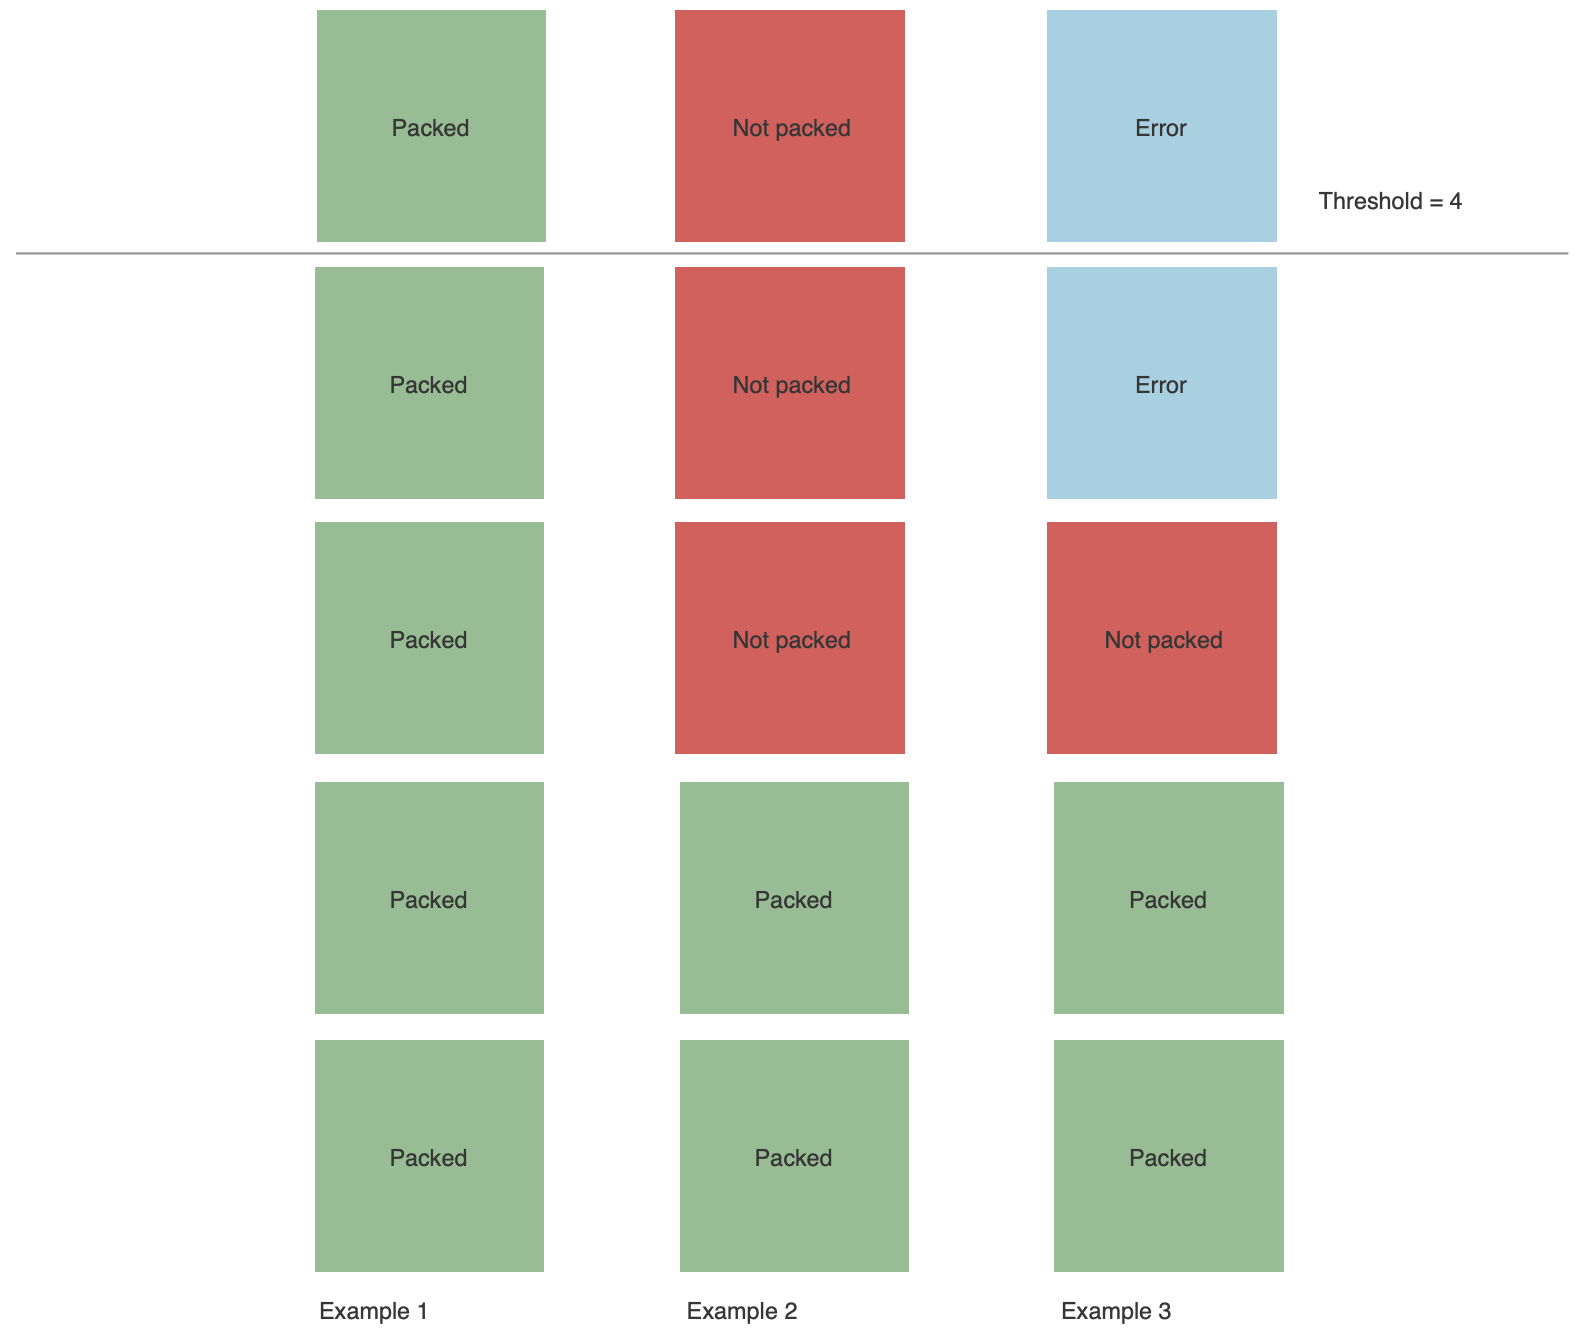
\includegraphics[width=0.8\linewidth]{Figures/error.png}
      \caption{Decisions with a threshold set to 4/5}
      \label{fig:error}
    \end{figure}
    The purpose of this test is thus to consider such \textit{errors} as \textit{packed} results and see if the overall performance is improved. Note that with this option enabled, the sample from example 3 now has a different label.
    \item \textbf{Agreement:} while the default consensus lies on the number of detectors that agree on the nature of a malware, i.e. packed or not packed, we also decided to observe how the dataset would change if they also had to agree on the same packer name. Table \ref{fig:agreement} illustrates this scenario.
    \begin{table}[H]
    \centering
    \begin{tabular}{|c|c|c|c|c|c|c|}
    \hline
     & Peframe & Manalyze & PEiD & DIE & Cisco & Decision \\
    \hline
     Default & UPX & none & UPX & PEtite & none & \textbf{packed} \\
     Agreement & UPX & none & UPX & PEtite & none & \textbf{not packed} \\
    \hline
    \end{tabular}
    \captionsetup{justification=centering}
    \caption{Decision with a threshold set to 3/5}
    \label{fig:agreement}
    \end{table}
    In the default situation, 3 detectors out of 5 agree on the nature of the sample. With a threshold of 3, the malware is then labeled as packed. For the agreement case, only 2 detectors agree on the same packer, namely UPX, which is less than 3. The final decision for the binary is then \textit{not packed}.
    
    Table \ref{Tab:others} gathers the results from the three previous scenarios, using all detectors and a threshold of 3/5. The second boolean test in the same as the first one where the 64 bytes following the EP are also converted.
    \begin{table}[H]
    \centering
    \resizebox{\textwidth}{!}{%
    \begin{tabular}{|c|c|c|c|c|c|}
    \hline
    Classifier & Default & Boolean1 & Boolean2 & Error as packed & Agreement\\
    \hline\hline
    KNN & \cellcolor{cyan}0.981 & \cellcolor{green}0.989 & \cellcolor{green}0.993 & \cellcolor{green}0.982 & \cellcolor{green}0.983 \\
    \hline
    GaussianNB & \cellcolor{cyan}0.907 & \cellcolor{green}0.915 & \cellcolor{green}0.974 & 0.900 & \cellcolor{green}0.908\\
    \hline
    BernoulliNB & \cellcolor{cyan}0.945 & 0.914 & \cellcolor{green}0.947 & 0.945 & \cellcolor{green}0.947\\
    \hline
    LogReg & \cellcolor{cyan}0.992 & 0.986 & \cellcolor{green}0.995 & 0.992 & 0.992\\
    \hline
    LinearSVC & \cellcolor{cyan}0.993 & 0.985 & 0.993 & 0.993 & 0.992\\
    \hline
    Decision Tree & \cellcolor{cyan}0.995 & 0.987 & 0.989 & 0.995 & 0.986\\
    \hline
    DL8.5 & \cellcolor{cyan}0.992 & 0.979 & 0.992 & 0.991 & 0.990\\
    \hline
    Gradient Boosted & \cellcolor{cyan}0.997 & 0.990 & 0.996 & 0.996 & 0.997\\
    \hline
    Random Forest & \cellcolor{cyan}0.994 & 0.979 & 0.994 & 0.994 & \cellcolor{green}0.995\\
    \hline
    MLP & \cellcolor{cyan}0.994 & 0.989 & \cellcolor{green}0.996 & \cellcolor{green}0.996 & \cellcolor{green}0.997\\
    \hline
    SVM & \cellcolor{cyan}0.995 & 0.989 & 0.995 & \cellcolor{green}0.996 & \cellcolor{green}0.996\\
    \hline
    \end{tabular}%
    }
    \captionsetup{justification=centering}
    \caption{Tests over datasets generated with boolean values, error as packed and agreement}
    \label{Tab:others}
    \end{table}
    The results we get are quite diversified, but some global conclusions can still be drawn. First, regarding the boolean scenarios, it seems pretty obvious that converting all features provides better outcomes than without the 64 additional byte values. However, using the second boolean conversion does not necessarily imply an increase in the prediction power for all classifiers, only for half of them, as shown by the green cells. Secondly, we can see that considering errors as packed only improved accuracy for less than 1/3 of the classifiers, and even when it did, the increase was minimal. Regarding the agreement, while also minor, it enhanced the prediction power for half of them. Agreement could then be kept but we rather not use the error as packed customisation since future models might learn fake information.
    
    To wrap up, while agreement is neutral or even beneficial for a few classifiers, complete boolean conversion might also be of interest but should be performed with care.
\end{itemize}

As a way to conclude this set of experiments, plot \ref{fig:final_results} gathers both accuracy and time for all classifiers according to their optimal combination of parameters, features, components and datasets. Training and testing have been performed over a dataset of 27 000 samples, which was the most we could get since Cisco was not able to provide us with further results at that time. Note that the running time for the DL8.5 is actually equal to the value chosen for the \texttt{time\_limit} parameter, which is 2 minutes, but for convenience it has been limited to 10 seconds on the graph.

\begin{figure}[!ht]
\centering
  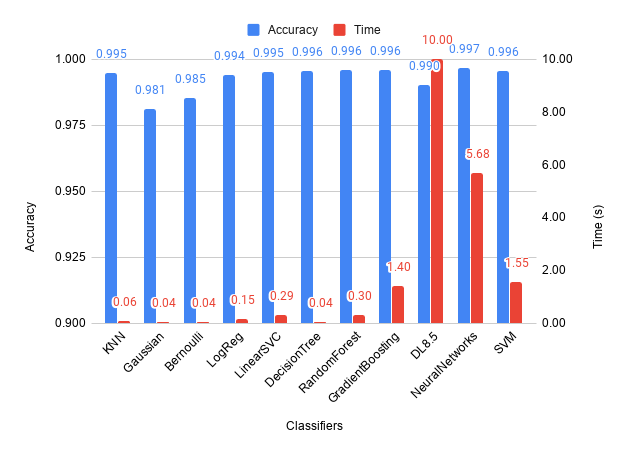
\includegraphics[width=\textwidth]{Figures/final_results.png}
  \captionsetup{justification=centering}
  \caption{Final test accuracies and time for all classifiers after complete customisation}
  \label{fig:final_results}
\end{figure}

Since the main goal of this whole machine learning section is to end up with one model that will be responsible for classifying further new samples, we decided to only keep a small subset of the classifiers for the next iteration. The last experiments are made to assess and refine the efficiency of the chosen classifiers to ease the final selection. By taking into account both time and accuracy, the four following models have been elected, each belonging to a different family of classifiers:  \textit{K-Nearest Neighbors}, \textit{Logistic Regression}, \textit{Decision Tree} and \textit{Random Forest}.

\subsection{Third phase: assertion tests}

\paragraph{Cross-validation}

One way to assert that the results we got from previous tests were not too specific to the training and test used is to proceed to cross-validation. Indeed, while using a training and test set is a common and correct approach to measure performance, we might be unlucky when splitting and have nearly all labels from one family in the training set and none of them in the test set. Therefore, the resulting accuracies might be promising but we are more likely to perform poorly when giving a new test set containing labels that were never encountered before. This is why we use cross-validation. It is a technique that evaluates generalisation performance where the input data is split repeatedly in different subsets and several models are trained. It then significantly enhances the probability to face each label in both the training and test set. The one we decided to go for is called \textit{k-fold} cross-validation, which means that the dataset will be divided into \textit{k} sections of equal size, called \textit{folds}. Then, \textit{k} models are trained where one section is used as the test set while the four other ones are gathered and used as the training test. This process is repeated so that each fold is used once as the test set. At the end, we have collected \textit{k} accuracy values and can compute a more representative mean value.

% \begin{figure}[!ht]
% \centering
%   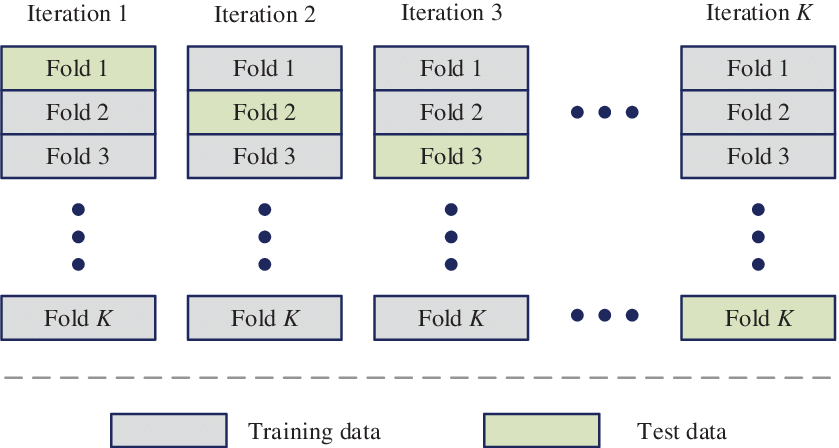
\includegraphics[width=\textwidth]{Figures/cross_validation.png}
%   \caption{Theoretical example of a K-fold cross-validation process \cite{cv_source}}
%   \label{fig:cross-validation}
% \end{figure}

Evaluating the 4 classifiers chosen at the end of the previous section with a \textit{5-fold cross-validation} over 27 000 samples, we got the following results:

\begin{table}[H]
    \centering
    \resizebox{\textwidth}{!}{%
     \begin{tabular}{|c|c|c|c|c|c|c|}
     \hline
     Classifier & Iteration 1 & Iteration 2 & Iteration 3 & Iteration 4 & Iteration 5 & \cellcolor{cyan}Mean\\
     \hline\hline
     KNN & 0.99389 & 0.99703 & 0.99315 & 0.99247 & 0.98759 & \cellcolor{cyan}0.99282\\
     \hline
     LogReg & 0.99445 & 0.99482 & 0.99593 & 0.99204 & 0.98926 & \cellcolor{cyan}0.99330\\ 
     \hline
     DecisionTree & 0.99482 & 0.99389 & 0.99315 & 0.99278 & 0.99 & \cellcolor{cyan}0.99293\\ 
     \hline
     RandomForest & 0.99593 & 0.99408 & 0.99704 & 0.99481 & 0.98926 & \cellcolor{cyan}0.99422\\ 
     \hline
    \end{tabular}%
    }
    \caption{Test accuracies obtained using 5-fold cross-validation}
    \label{Tab:k_fold}
\end{table}

Since, in average, all accuracies are still around 99\% of precision, we can assert that the models were not overfitting and generalise pretty well.

\paragraph{Economical analysis}

For this last experience, Cisco was not able to provide us with the results from its new analysis. If only considering their previous outcomes, we could just create a dataset of around 30 000 malware. Therefore, we decided to drop Cisco's results at this point and managed to produce a dataset containing more than 140 000 samples. The threshold used was therefore the most restraining possible, namely 4/4. Statistics about this adapted ground truth can be found in \autoref{gt_stats}.

Economical analysis is a process where the stability of our classifiers is assessed over time. The idea is to train the models over a certain period of time and then test them over completely new input data. Doing this allows to observe if classifiers can generalise well over possibly new kinds of malware.

In order to make it as modular as possible with further bigger datasets, we decided to apply economical analysis as follows: when given a dataset, it is first divided into 6 different sections of equal size \textit{S}, called \textit{periods}. Then, tuning and learning is applied to half of the dataset, so 3 out of 6 splits. Eventually, the 3 last sections are individually used as the test set. Doing this mimics the learning over different new periods of time, since each test set is \textit{S} samples older than its predecessor. Since the ground truth has been continuously updated with newer malware, we are more likely to encounter different kinds of malware in the last periods. 

Proceeding to economical analysis with our selection of best classifiers, we obtained the test accuracies shown in table \ref{Tab:eco_analysis}.

\begin{table}[H]
    \centering
    \resizebox{\textwidth}{!}{%
     \begin{tabular}{|c|c|c|c|c|c|c|}
     \hline
     Classifier & 1 period old & 2 periods old & 3 periods old \\
     \hline\hline
     KNN & 0.994199 & 0.990485 & 0.993405\\
     \hline
     LogReg & 0.99278 & 0.992863 & 0.990775\\ 
     \hline
     DecisionTree & 0.994032 & 0.994449 & 0.992111\\ 
     \hline
     RandomForest & 0.990485 & 0.986228 & 0.988521\\ 
     \hline
    \end{tabular}%
    }
    \captionsetup{justification=centering}
    \caption{Test accuracies collected from running economical analysis over the KNN, LogReg, Decision Tree and Random Forest classifier}
    \label{Tab:eco_analysis}
\end{table}

As a general conclusion, it can be observed that our selection of models managed to keep a stable performance when predicting over new input data, positioned around 99\%. On the other hand, we cannot really identify some kind of general behavior since accuracies are not simply decreasing over time for every classifier. The reason why performance are sometimes better for the third period than for the second one could be because an older malware has regain popularity or because a new version has been released, allowing our classifiers to find common features and detect it anyway.
We can also highlight that while the prediction power of the Random Forest classifier decreases slightly with new input until falling below 99\% of precision, the Decision Tree model keeps a test accuracy between 99.21 and 99.45\%, and even improves over the second period. While these behaviors could be certified - or not - using even more samples - of which we do not dispose of at the moment - the current results we gathered are enough to confirm that the selection of classifiers made previously can keep suitable results for a decent amount of time. However, if we had to keep only one of them, we would probably go for the Decision Tree model. This is because of its standard deviation of only 0.2\% combined with its training time being faster than its peers.